\documentclass{codeclass}

\title{Atividade 2}
\author{\texorpdfstring{$\Jimeens\limits_{({\color{red!70!black}11917239})}$}{}}
\affiliation{Instituto de Física, \href{https://ror.org/036rp1748}{Universidade de São Paulo}, Rua do Matão 1371, 05508-090, Cidade Universitária, São Paulo, Brasil} % Affiliation
\dated{\today}

\abstract{Fazer uma análise de regressão supervisionada para determinar a temperatura crítica de materiais. Utilizar diferentes modelos e subconjuntos de dados, comparando o desempenho e a interpretabilidade.

\rule{\linewidth}{1pt}

Comentário: Em um repositório no Github salvei um arquivo nomeado \verb|Atividade2.ipynb|, contendo as mesmas informações e comentários presentes neste PDF, então para tornar a correção possivelmente mais simples, os arquivos estão contidos nos \textit{shields} abaixo, basta clicar em qual arquivo é mais simples de verificar.

\begin{center}
    \drawBadge[ labelColor=black,
                color=red!70!black, 
                logo=\colab, link=https://colab.research.google.com/github/Jimeens/PGF5393_IA/blob/main/Atividade2.ipynb]
                {}{Abrir No Colab}
    \drawBadge[ labelColor=black,
                color=red!70!black, 
                logo=\faGithub, link=https://github.com/Jimeens/PGF5393_IA/blob/1c187eff72991ee9232132643e0fdf7381948952/Atividade2.ipynb]
                {}{Abrir no GitHub}
\end{center}}

\begin{document}

\maketitle

\section{Análise exploratória}

    

Iniciamos nossa análise importando os dados dos arquivos \href{https://raw.githubusercontent.com/Jimeens/Permanent_Files/refs/heads/main/PGF5393/Atividade1/Stars.csv}{\texttt{Stars.csv}} e \href{https://raw.githubusercontent.com/Jimeens/Permanent_Files/refs/heads/main/PGF5393/Atividade1/Categorias.csv}{\texttt{Categorias.csv}}. Para isso, importamos a biblioteca \verb|pandas|
\begin{longlisting}
    \begin{minted}{py}
        import pandas as pd

        dS = pd.read_csv('Stars.csv')
        dC = pd.read_csv('Categorias.csv')

        dS
    \end{minted}
\end{longlisting}

Podemos ver que a tabela \verb|dS| possui as seguintes variáveis
\begin{table}[H]
    \centering
    \begin{tabular}{cccccccc}
        \toprule
        \verb|index| & \verb|Star| & \verb|Temperature| & \verb|L| & \verb|R| & \verb|A_M| & \verb|Color| & \verb|Spectral_Class| \\ 
        \midrule
        0 & 1 & 3068 & 0.002400 & 0.1700 & 16.12 & Red & M \\
        1 & 2 & 3042 & 0.000500 & 0.1542 & 16.60 & Red & M \\
        2 & 3 & 2600 & 0.000300 & 102.0000 & 18.70 & Red & M \\
        3 & 4 & 2800 & 0.000200 & 0.1600 & 16.65 & Red & M \\
        4 & 5 & 1939 & 0.000138 & 103.0000 & 20.06 & Red & M \\
        $\cdots$ & $\cdots$ & $\cdots$ & $\cdots$ & $\cdots$ & $\cdots$ & $\cdots$ & $\cdots$ \\
        235 & 236 & 38940 & 374830.000000 & 1356.0000 & -9.93 & Blue & O \\
        236 & 237 & 30839 & 834042.000000 & 1194.0000 & -10.63 & Blue & O \\
        237 & 238 & 8829 & 537493.000000 & 1423.0000 & -10.73 & White & A \\
        238 & 239 & 9235 & 404940.000000 & 1112.0000 & -11.23 & White & A \\
        239 & 240 & 37882 & 294903.000000 & 1783.0000 & -7.80 & Blue & O \\
        \bottomrule
    \end{tabular}
\end{table}

Antes de começar a preparar os dados, uma verificação curial é em relação à existência ou não valores ausentes nas duas tabelas, pois caso exista algum, é necessário fazer uma análise a mais nos dados. Na tabela \verb|dS|:
\begin{longlisting}
    \begin{minted}{py}
        print("Valores ausentes na tabela Stars.csv:")
        print(dS.isnull().sum())
    \end{minted}
\end{longlisting}
\begin{verbatim}
    Valores ausentes em Stars.csv:
    Temperature       0
    L                 0
    R                 0
    A_M               0
    Color             0
    Spectral_Class    0
\end{verbatim}
e na tabela \verb|dC|:
\begin{longlisting}
    \begin{minted}{py}
        print("Valores ausentes em Categorias.csv:")
        print(dC.isnull().sum())
    \end{minted}
\end{longlisting}
\begin{verbatim}
    Valores ausentes em Categorias.csv:
    Star    0
    Type    0
\end{verbatim}

Concluindo que não existem valores ausentes em nenhuma delas e portanto a análise pode ser desenvolvida diretamente.

Ao olha para tabela, vemos que a coluna \verb|Star| é um identificador desnecessário, de modo que para anonimizar os dados, removemos esta coluna. Além disso, temos 4 variáveis numéricas (\verb|Temperature|, \verb|L|, \verb|R| e \verb|A_M|) e 2 variáveis categóricas (\verb|Color| e \verb|Spectral_Class|), tal que podemos separá-las em duas listas independentes.
\begin{longlisting}
    \begin{minted}{py}
        dS = dS.drop(columns = ['Star'])

        varNum = ['Temperature', 'L', 'R', 'A_M'] 
        varCat = ['Color', 'Spectral_Class'] 
    \end{minted}
\end{longlisting}

Em relação às variáveis numéricas, pode-se notar uma grande variação de escala nos dados, isto é, a variável \verb|Temperature| $\in[1939, 40000]$, a variável \verb|L| $\in[0.000080, 849420.0]$, a variável \verb|R| $\in [0.008400, 6237.0]$ e a variável \verb|A_M| $\in [-7346.0, 14776.0]$. 
\begin{longlisting}
    \begin{minted}{py}
        dS.describe()
    \end{minted}    
\end{longlisting}
\begin{table}[H]
    \centering
    \begin{tabular}{ccccc}
        \toprule
        \verb|index| & \verb|Temperature| & \verb|L| & \verb|R| & \verb|A_M|  \\ 
        \midrule
        count & 240.000000 & 240.000000 & 240.000000 & 240.000000 \\
        mean & 10497.462500 & 107200.578572 & 415.982944 & 121.369458 \\
        std & 9552.425037 & 179424.946945 & 963.239600 & 2089.328079 \\
        min & 1939.000000 & 0.000080 & 0.008400 & -7346.000000 \\
        25\% & 3344.250000 & 0.000865 & 0.195025 & -6.342500 \\
        50\% & 5776.000000 & 7.960000 & 18.000000 & 10.515000 \\
        75\% & 15055.500000 & 198050.000000 & 277.500000 & 14.097500 \\
        max & 40000.000000 & 849420.000000 & 6237.000000 & 14776.000000 \\
        \bottomrule
    \end{tabular}
\end{table}

Esta grande variação de escala sugere um reescalonamento destes dados, o que será comentado em mais detalhes no item 2. 

Uma análise inicial a ser feita é em relação à variável \verb|A_M|. Em relação aos dados presentes nesta coluna, aproximadamente 95\% possui duas casas decimais e estão em torno de um intervalo $[-10, 20]$, porém, existem alguns dados que são $> 100$ e $< -100$ ($|$\verb|A_M|$|$ $> 100$), que são números inteiros maiores que 1000, o que sugere uma inconsistência nestes valores. Para isso importamos a biblioteca \verb|numpy|
\begin{longlisting}
    \begin{minted}{py}
        import numpy as np
        
        bigA_M = np.abs(dS['A_M'])
        countBigA_M = (bigA_M > 100).sum()
        
        print(f"{100 * (240 - countBigA_M)/240:.3f}% estão abaixo de |A_M|<100")
        bigA_MStars = dS[bigA_M > 100][['A_M']]
    \end{minted}
\end{longlisting}
\begin{verbatim}
    94.583% estão abaixo de |A_M|<100
\end{verbatim}
\begin{table}[H]
    \centering
    \begin{tabular}{cc}
        \toprule
        \verb|index| & \verb|A_M|  \\ 
        \midrule
        14 & 11782.0 \\
        91 & 6506.0 \\
        92 & 6228.0 \\
        161 & -6245.0 \\
        193 & 12854.0 \\
        195 & 13667.0 \\
        199 & 14776.0 \\
        216 & 1236.0 \\
        223 & -5975.0 \\
        226 & -7262.0 \\
        227 & -6224.0 \\
        228 & -5905.0 \\
        229 & -7346.0 \\
        \bottomrule
    \end{tabular}
\end{table}

Para corrigi-los, impomos uma condição de divisão por um fator $1000$. 
\begin{longlisting}
    \begin{minted}{py}
        dS['A_M'] = np.where(np.abs(dS['A_M']) > 100, dS['A_M'] / 1000, dS['A_M'])
    \end{minted}
\end{longlisting}

Em relação às variáveis categóricas, há uma inconsistência nos dados da variável \verb|Color|. Existem dados que representam a mesma categoria, mas que estão escritas de forma diferente, por exemplo, a opção \verb|Blue Color| pode ser encontrada também nas formas \verb|Blue-Color|, \verb|Blue-color| e \verb|Blue color|, o que pode gerar inconsistências futuras na hora de analisar os dados. Faremos então um remapeamento desta variável levando em conta inconsistências de escrita e, como estamos lidando com cores, proximidades de tons.
\begin{longlisting}
    \begin{minted}{py}
        color_map = {
            'Red': 'Red',
            'Orange': 'Orange',
            'Orange-Red': 'Orange',
            'Pale yellow orange': 'Orange',
            'Yellowish': 'Yellow',
            'yellowish': 'Yellow',
            'Yellowish White': 'Yellowish_White',
            'yellow-white': 'Yellowish_White',
            'White-Yellow': 'Yellowish_White',
            'Whitish': 'White',
            'White': 'White',
            'white': 'White',
            'Blue': 'Blue',
            'Blue White': 'Blue_White',
            'Blue white': 'Blue_White',
            'Blue-white': 'Blue_White',
            'Blue-White': 'Blue_White'
        }
        dS['Color'] = dS['Color'].map(color_map).fillna(dS['Color'])
    \end{minted}
\end{longlisting}

Com este remapeamento, podemos verificar que o número de tipos de \verb|Color| e a quantidade de \verb|Spectral_Class| são os mesmos e que devem possuir uma forte correlação, pois as quantidades são muito similares, principalmente para \verb|Color = Red| e \verb|Color = Blue_White|, que possuem muitos dados. Podemos então assumir que como uma é equivalente à outra, uma das duas colunas pode ser descartada para simplificação da análise. Neste caso, como os dados de \verb|Color|, originalmente, são inconsistentes e são relativamente difíceis de lidar, pois o nome de uma cor pode ser vista de diversas formas diferentes (ex.: considerar o que é laranja amarelado, laranja e laranja avermelhado acaba sendo um pouco complicado, pois não conseguimos de fato separar o que é mais laranja, mais amarela ou mais vermelho apenas olhando), pode ser interessante retirar esta coluna, de modo que a tabela \verb|dS| vai possuir apenas as colunas \verb|Temperature|, \verb|L|, \verb|R|, \verb|A_M| e \verb|Spectral_Class|.
\begin{longlisting}
    \begin{minted}{py}
        dS = dS.drop(columns = ['Color'])
    \end{minted}
\end{longlisting}

% Levando em consideração que iremos utilizar o método PCA e faremos uma clusterização, é necessário converter os dados categóricos em valores numéricos, o que pode ser feito utilizando o codificador \verb|OneHotEncoder(sparse_output = False)| da biblioteca \verb|sklearn|, cujo argumento interno ao codificador é usado para retornar uma matriz densa (\textit{dense array}) onde todos os valores (0 ou 1) são explicitamente armazenados.
Levando em conta que iremos utilizar o método PCA e formaremos \textit{clusters}, é necessário converter os dados categóricos remanescentes na tabela em valores numérico. Então, para realizar a conversão da variável \verb|Spectral_Class|, podemos utilizar o codificador \verb|OneHotEncoder(sparse_output = False)| da biblioteca \verb|sklearn|, cujo argumento interno é usado para retornar uma matriz densa onde todos os valores binários são explicitamente armazenados.
% \begin{longlisting}
%     \begin{minted}{py}
%         from sklearn.preprocessing import OneHotEncoder
        
%         encoder = OneHotEncoder(sparse_output=False) 
%         encodedCat = encoder.fit_transform(dS[varCat])
%         encodeddS = pd.DataFrame(encodedCat, columns=encoder.get_feature_names_out(varCat))

%         encodeddS
%     \end{minted}
% \end{longlisting}
\begin{longlisting}
    \begin{minted}{py}
        from sklearn.preprocessing import OneHotEncoder

        encoder = OneHotEncoder(sparse_output=False)
        encodedClass = encoder.fit_transform(dS[['Spectral_Class']])
        encodeddS = pd.DataFrame(encodedClass, columns=encoder.get_feature_names_out())
    \end{minted}
\end{longlisting}
onde \verb|encodeddS| vai retornar uma tabela com 240 linhas e 7 colunas, e cada coluna vai ser um dos tipos das \verb|Spectral_Class|.
\begin{table}[H]
    \centering
    \begin{tabular}{cccccc}
        \toprule
        \verb|index| & \verb|Spectral_Class_A| & \verb|Spectral_Class_B| & $\cdots$ & \verb|Spectral_Class_M| & \verb|Spectral_Class_O|  \\ 
        \midrule
        0 & 0.0 & 0.0 & $\cdots$ & 1.0 & 0.0  \\
        1 & 0.0 & 0.0 & $\cdots$ & 1.0 & 0.0  \\
        2 & 0.0 & 0.0 & $\cdots$ & 1.0 & 0.0  \\
        3 & 0.0 & 0.0 & $\cdots$ & 1.0 & 0.0  \\
        4 & 0.0 & 0.0 & $\cdots$ & 1.0 & 0.0  \\
        $\cdots$ & $\cdots$ & $\cdots$ & $\cdots$ & $\cdots$ & $\cdots$ \\
        235 & 0.0 & 0.0 & $\cdots$ & 0.0 & 1.0  \\
        236 & 0.0 & 0.0 & $\cdots$ & 0.0 & 1.0  \\
        237 & 1.0 & 0.0 & $\cdots$ & 0.0 & 0.0  \\
        238 & 1.0 & 0.0 & $\cdots$ & 0.0 & 0.0  \\
        239 & 0.0 & 0.0 & $\cdots$ & 0.0 & 1.0  \\
        \bottomrule
    \end{tabular}
\end{table}

\section{Preparação dos dados: escalonamento, transformação, particionamento}

    \lipsum[1]

\section{Avaliar a importância dos atributos com base nos coeficientes de um modelo de regressão linear múltipla (com ou sem regularização, à sua escolha)}

    \lipsum[1]

\section{Avaliar a importância dos atributos com base em um regressor Random Forest ou Gradient Boosting}

    Escolhendo um regressor Random Forest pra avaliar a importância dos atributos, importamos a função \verb|RandomForestRegressor| do \verb|sklearn|. Da mesma forma que fizemos para determinar o melhor \verb|alpha| na função Ridge, podemos determinar o melhor \verb|n_estimators| da função \verb|RandomForestRegressor| com o \verb|GridSearchCV|. Como o custo computacional pra encontrar esse valor otimizado é muito alto, é preferível definir uma profundidade máxima do Random Forest (que escolho como sendo 10).
\begin{longlisting}
    \begin{minted}{python}
    %%time
    from sklearn.ensemble import RandomForestRegressor

    RFR = RandomForestRegressor(random_state=42)
    paramGrid = { 'n_estimators': [150, 250, 350],
                'max_depth': [None, 20, 40],
                'min_samples_leaf': [1, 2, 4]}

    gridSearch = GridSearchCV(RFR, paramGrid, cv=3, scoring='neg_mean_squared_error', n_jobs=-1, verbose=1)
    gridSearch.fit(XTrain, yTrain)

    bestEstimators = gridSearch.best_params_['n_estimators']
    bestDepth = gridSearch.best_params_['max_depth']
    bestLeaf = gridSearch.best_params_['min_samples_leaf']

    print("Melhor n_estimators:", bestEstimators)
    print("Melhor max_depth:", bestDepth)
    print("Melhor min_samples_leaf:", bestLeaf)
    \end{minted}
\end{longlisting}
\begin{verbatim}
    Fitting 3 folds for each of 27 candidates, totalling 81 fits
    Melhor n_estimators: 250
    Melhor max_depth: 20
    Melhor min_samples_leaf: 1
    CPU times: user 6min 30s, sys: 13.8 s, total: 6min 44s
    Wall time: 3h 49min 2s
\end{verbatim}

Ao verificar os melhores hiperparâmetros selecionados para o Radom Forest, foi determinado após (3h 49min 2s) que o melhor valor de \verb|n_estimators = 350|, o melhor de \verb|max_depth = 20| e o melhor de \verb|min_samples_leaf = 1|. Como o código acima demora muito tempo pra ser executado, após confirmar os valores, torno essa parte do programa um comentário e salvo os melhores valores separadamente.
\begin{longlisting}
    \begin{minted}{python}
    bestEstimators = 350
    bestDepth = 20
    bestLeaf = 1
    \end{minted}
\end{longlisting}
\begin{longlisting}
    \begin{minted}{python}
    RFR = RandomForestRegressor(max_depth=bestDepth, min_samples_leaf=bestLeaf, n_estimators=bestEstimators, random_state=42)
    RFR.fit(XTrain, yTrainLog)
    yPredRFR = RFR.predict(XTest)

    importances = pd.Series(RFR.feature_importances_, index=X.columns)
    print(importances.sort_values(ascending=False).head(10))
    \end{minted}
\end{longlisting}
\begin{verbatim}
    range_ThermalConductivity        0.604150
    mean_Density                     0.052367
    wtd_gmean_ThermalConductivity    0.038381
    wtd_mean_atomic_mass             0.015584
    wtd_std_ElectronAffinity         0.015372
    wtd_gmean_ElectronAffinity       0.013949
    wtd_mean_ThermalConductivity     0.010111
    range_atomic_radius              0.009012
    std_ThermalConductivity          0.008445
    wtd_gmean_Valence                0.008275
    dtype: float64
\end{verbatim}

Aqui as variáveis obtidas pelo Random Forest vão ser aquelas que reduzem a variância na predição.
\begin{longlisting}
    \begin{minted}{python}
    mseRFR = mean_squared_error(yTestLog, yPredRFR)
    r2RFR = r2_score(yTestLog, yPredRFR)

    print("MSE:", mseRFR)
    print("R²:", r2RFR)
    \end{minted}
\end{longlisting}
\begin{verbatim}
    MSE: 0.11751767353522158
    R²: 0.9296492860335409
\end{verbatim}

Vemos então que $R^{2} \approx 93.0\%$ a variância da temperatura crícita (em escala logaritmica) pode ser explicada pelas variáveis selecionadas pelo modelo. No caso do erro médio quadrático, se determinarmos o RMSE e exponenciarmos, vamos obter algo como $\exp(\sqrt{\text{MSE}}) \approx 1.41$, indicando um erro multiplicativo ainda menor do que o obtido na regressão linear.

\section{Com base nos resultados dos itens 3 e 4, selecionar os atributos mais importantes. O número de atributos fica à sua escolha. Justificar sua escolha. Discutir brevemente se os atributos possuem significado físico, ou seja, se de fato pode existir uma relação com a variável alvo (temperatura crítica)}

    

A fim de utilizar o método de agrupamento hierárquico para agrupar as estrelas, podemos descobrir o número de agrupamentos ideal para análise de dados via \verb|AgglomerativeClustering|, de modo que num \textit{range} de 2 a 11 \textit{clusters}, podemos visualizar qual é este valor ideal de \textit{clusters}.
\begin{longlisting}
    \begin{minted}{py}
        from sklearn.cluster import AgglomerativeClustering
        from sklearn.metrics import silhouette_score, silhouette_samples
        
        silHier = []
        for n in range(2, 11):
            hier = AgglomerativeClustering(n_clusters=n, linkage='ward')
            labels = hier.fit_predict(scaledNumdS)
            silHier.append(silhouette_score(scaledNumdS, labels))
        
        plt.plot(range(2,11), silHier, marker='o')
        plt.xlabel('Número de Clusters')
        plt.ylabel('Fator de Silhoueta')
        plt.show()
    \end{minted}
\end{longlisting}
\begin{figure}[H]
    \centering
    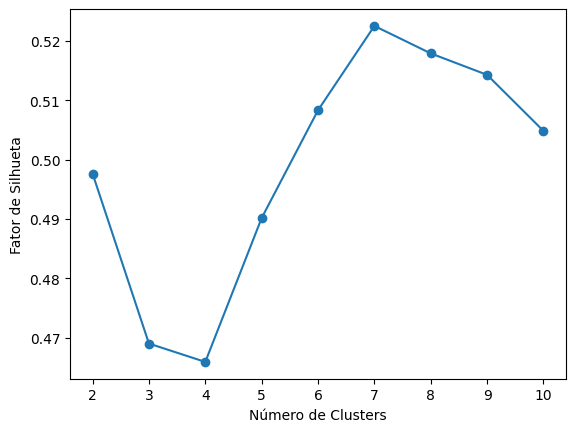
\includegraphics[width=0.5\linewidth]{figures/HierClustSilhouette.png}
\end{figure}
cujo número ideal de \textit{clusters} vai ser definido pelo maior fator de silhueta observado no gráfico, o que podemos gravar no comando
\begin{longlisting}
    \begin{minted}{py}
        bestNumberClustersHier = list(range(2,11))[np.argmax(silHier)]
    \end{minted}
\end{longlisting}
que, para este caso, guardará o valor \verb|bestNumberClusterHier = 7|. Com isso podemos agrupar as estrelas em 7 \textit{clusters}, de tal forma que os gráficos relacionando as características principais das estrelas são facilmente construídos.
\begin{longlisting}
    \begin{minted}{py}
        hierarchical = AgglomerativeClustering(n_clusters=bestNumberClustersHier, linkage='ward').fit(scaledNumdS)
        categoriasHier = hierarchical.labels_

        plt.figure(figsize=(15,10))
        for i, (xVar, yVar) in enumerate([('Temperature', 'L'), ('R','A_M'), ('Temperature','R'), ('L','A_M'), ('Temperature', 'A_M'), ('R','L')], 1):
            plt.subplot(2,3,i)
            plt.scatter(scaledNumdS[xVar], scaledNumdS[yVar], c=categoriasHier, cmap='inferno')
            plt.xlabel(xVar)
            plt.ylabel(yVar)
    \end{minted}
\end{longlisting}
\begin{figure}[H]
    \centering
    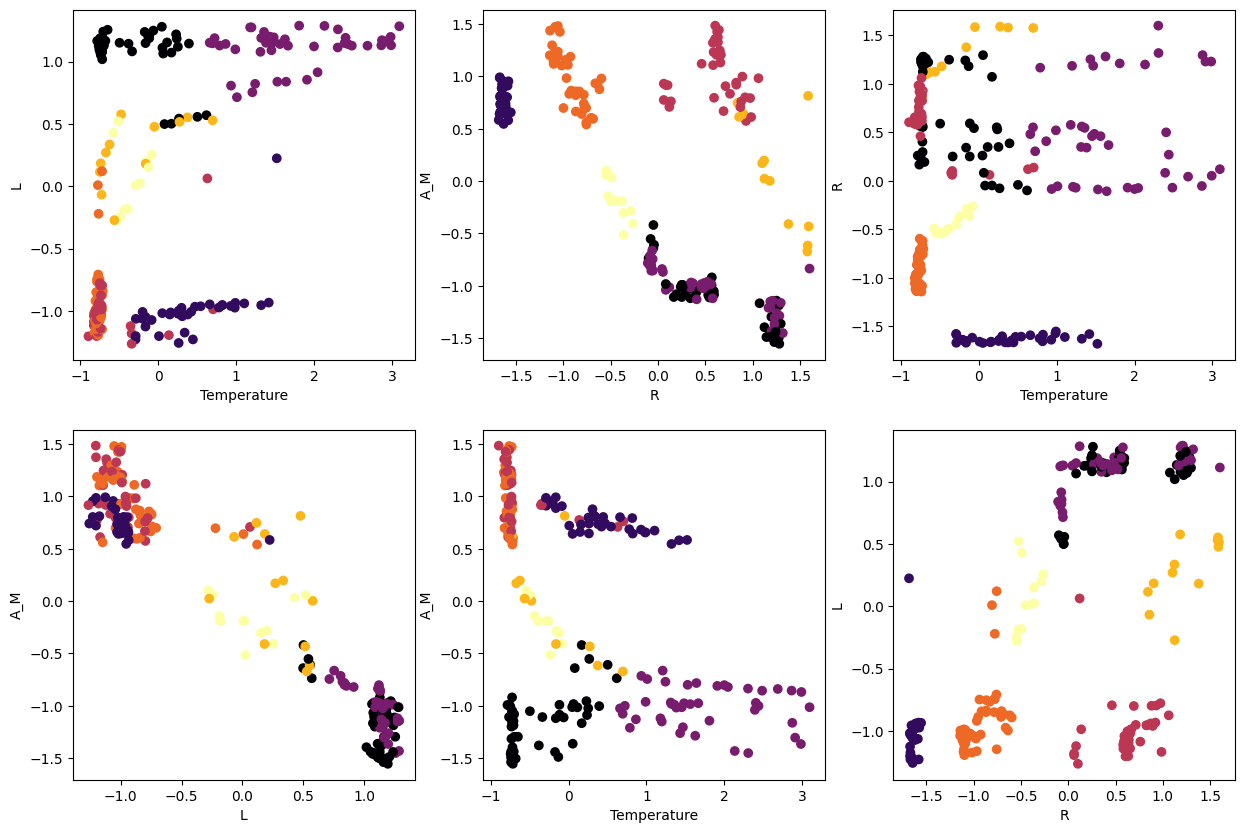
\includegraphics[width=\linewidth]{figures/Hierarchical.png}
\end{figure}

% O método de agrupamento hierárquico mostra uma clusterização interessante ao olharmos principalmente para os gráficos de \verb|A_M| $\times$ \verb|R|, \verb|A_M| $\times$ \verb|Temperature| e \verb|L| $\times$ \verb|R|, pois mesmo que a visualização não seja tão clara, conseguimos ver alguns \textit{clusters} bem formados e separados


\section{Aplicar uma técnica de redução de dimensionalidade, como PCA (análise de componentes principais), criando novos atributos a partir de uma combinação dos atributos originais. O número de componentes principais a serem utilizadas fica à sua escolha (justificar escolha)}

    \lipsum[1]

\section{Construir um modelo de regressão linear múltipla com: a) os atribuutos mais importantes, escolhidos no item 5; b) usando as componentes principais como atributos (item 6). Comparar o desempenho desses modelos na predição da temperatura crítica e a sua inteerpretabilidade (isto é, se é fácil ou não interpretar o significado físico dos coeficientes ajustados). Avalie se o modelo é capaz de predizer diferentes faixas de valores de temperatura crítica}

    \lipsum[1]

\section{Construir um modelo de regressão baseado em Random Forest ou Gradient Boosting com: a) apenas os atributos mais importantes, escolhidos no item 5; b) usando as componentes principais como atributos (item 6). Lembre-se de otimizar os hiperparâmetros. Comparar o desempenho desses modelos na predição da temperatura crítica e sua interpretabilidade. Avalie se o modelo é capaz de predizer diferentes faixas de valores de temperatura crítica}

    

As categorias definidas manualmente na tabela \verb|dC| podem ser visualizadas em \textit{clusters}, onde cada tipo da variável \verb|Type| vai definir um \textit{cluster}, de modo que a visualização pode ser feita utilizando a biblioteca \verb|seaborn|.
\begin{longlisting}
    \begin{minted}{py}
        import seaborn as sns

        plt.figure(figsize=(15, 10))
        for i, (x_feature, y_feature) in enumerate([('Temperature', 'L'), ('R', 'A_M'), ('Temperature', 'R'), ('L', 'A_M'), ('Temperature', 'A_M'), ('R', 'L')], 1):
            plt.subplot(2, 3, i)
            sns.scatterplot(x=x_feature, y=y_feature, hue=dC['Type'], data=scaledNumdS, palette='inferno')
    \end{minted}
\end{longlisting}
\begin{figure}[H]
    \centering
    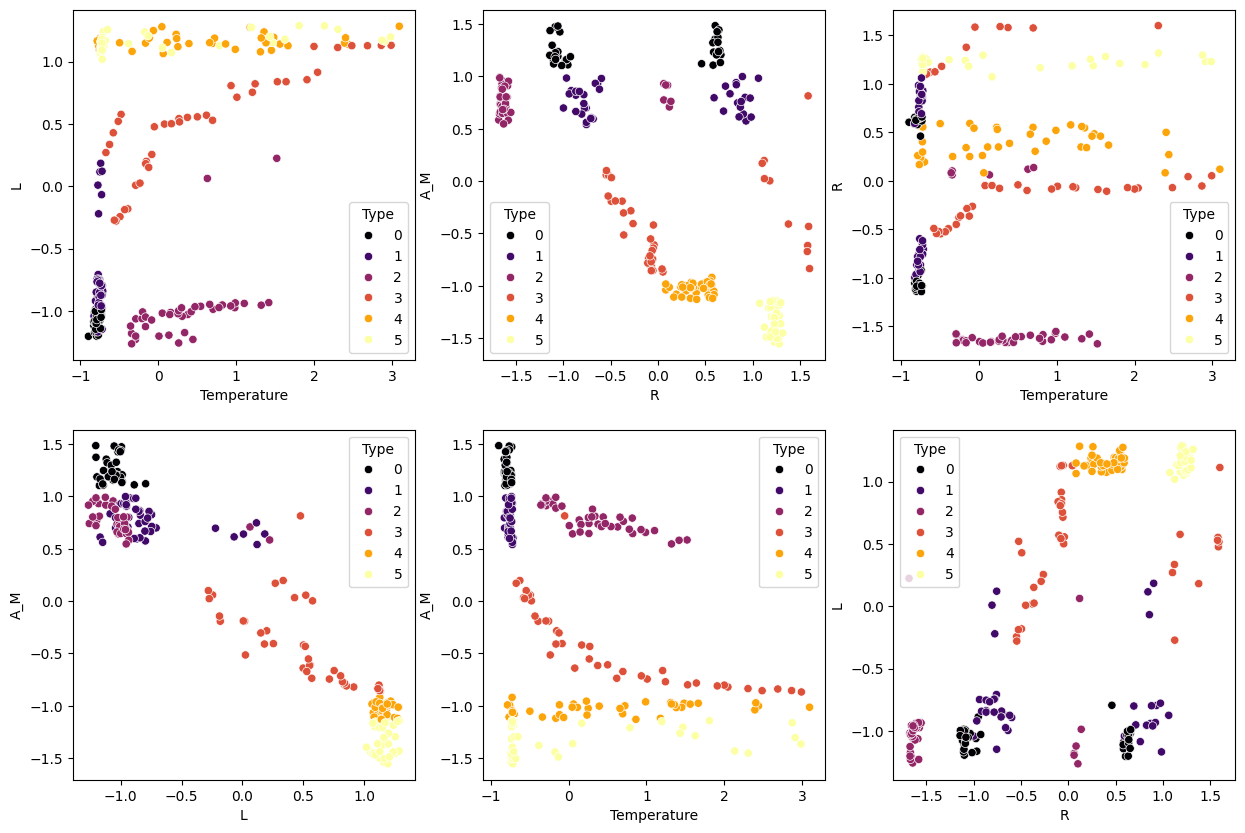
\includegraphics[width=1\linewidth]{figures/Manual.png}
\end{figure}

Vemos aqui que os \textit{clusters} são muito bem separados e de clara visualização. Em comparação com os agrupamentos feitos com agrupamento Hierárquico, KMeans e DBSCAN, podemos verificar o quão parecido os \textit{clusters} são utilizando a métrica \textit{Adjusted Rand Index} (ARI).
\begin{longlisting}
    \begin{minted}{py}
        from sklearn.metrics import adjusted_rand_score

        ariHierarchical = adjusted_rand_score(dC['Type'], categoriasHier)
        ariKMeans = adjusted_rand_score(dC['Type'], categoriasKMeans)
        ariDBSCAN = adjusted_rand_score(dC['Type'], categoriasDBSCAN)
        
        print(f'ARI Hierárquico: {ariHierarchical:.3f}')
        print(f'ARI KMeans: {ariKMeans:.3f}')
        print(f'ARI DBSCAN: {ariDBSCAN:.3f}')
    \end{minted}
\end{longlisting}
\begin{verbatim}
    ARI Hierárquico: 0.396
    ARI KMeans: 0.397
    ARI DBSCAN: 0.406
\end{verbatim}

Podemos ver então que os \textit{clusters} formados pelos métodos de agrupamento hierárquico, KMeans e DBSCAN são relativamente inferiores (DBSCAN $>$ KMeans $>$ Hierárquico) quando comparados às categorias definidas manualmente, no entanto, alguns \textit{clusters} obtidos por estes métodos são relativamente parecidos com os manuais.

Um comentário importante a ser feito é em relação ao uso do \verb|random_state=2|no KMeans. Ao impormos isso, a \textit{clusterização} fica única, porém ela pode não ser a melhor formação de \textit{clusters} quando fazemos \verb|kmeans = KMeans(n_clusters=bestNumberClustersKMeans, random_state=2).fit(scaledNumdS)|, dado que existe uma variedade de \verb|random_state| que nos dão um valor ótimo de \textit{clusters} igual a 6, mas todos eles acabam por ser diferentes e o ARI do KMeans vai sempre mudar.

\section{Fazer uma breve discussão crítica sobre o desempenho, a interpretabilidade e o custo computacional dos modelos lineares e dos modelos baseados em árvores de decisão}

    Ao olharmos para o fator desempenho dos modelos, temos que os modelos baseados em árvores de decisão, neste caso o Random Forest, são mais eficientes em relação à previsibilidade da temperatura crítica, porém o custo computacional é extremamente maior, mesmo considerando menos atributos. Quando otimizamos os hiperparâmetros do Random Forest utilizando o \verb|GridSerchCV| com todos os atributos, o custo computacional foi da ordem de $\sim 4$ horas, o que muitas vezes acaba sendo inviável, então reduzir a dimensionalidade dos atributos considerados em aproximadamente $4$ vezes reduziu esse custo quase em $4$ vezes também, mas ainda sendo muito mais custoso que um modelo linear de regressão.

Utilizando a redução de dimensionalidade das componentes principais, conseguimos predizer de forma consideravelmente boa os valores de temperatura crítica, porém acabamos perdendo a interpretabilidade física, pois cada componente principal vai utilizar de combinações lineares dos atributos originais diferentes, o que muitas vezes pode não ser muito bom, pois perdemos informações importantes, como o tipo de relação que um certo atributo terá com a temperatura crítica.

Podemos então concluir que os modelos de árvore de decisão são mais adequados para determinar a temperatura crítica dos materiais, principalmente considerando o caso onde consideramos apenas 14 dos 81 atributos originais, como feito no item 8.(a).

\end{document}